\subsection{Hyperparamters}

Through grid search the best combination of $\lambda$- and degree-values where found to be: 

\begin{table}[h!]
    \centering
    \begin{tabular}{|c|c|c|c|}
        \hline
        & & \textbf{Franke Function} & \textbf{Terrain Data} \\ \hline
        \textbf{Ridge} & $\lambda$ & 2.4 $\times 10^{-2}$ & 3.0 $\times 10^{-5}$ \\ 
         & degree & 7 & 4 \\ \hline
        \textbf{Lasso} & $\lambda$ & 1.7 $\times 10^{-5}$ & 2.2 $\times 10^{-4}$ \\ 
         & degree & 7 & 6 \\ \hline
    \end{tabular}
    \caption{Best pairs of $\lambda$- and degree values found through grid search}
    \label{tab:grid}
\end{table}

In the following sections, the Lasso- and Ridge regression models are trained with their respective $\lambda$ values from Tab. \ref{tab:grid}. 

\subsection{Franke function}

\begin{figure}[h!]
    \centering
    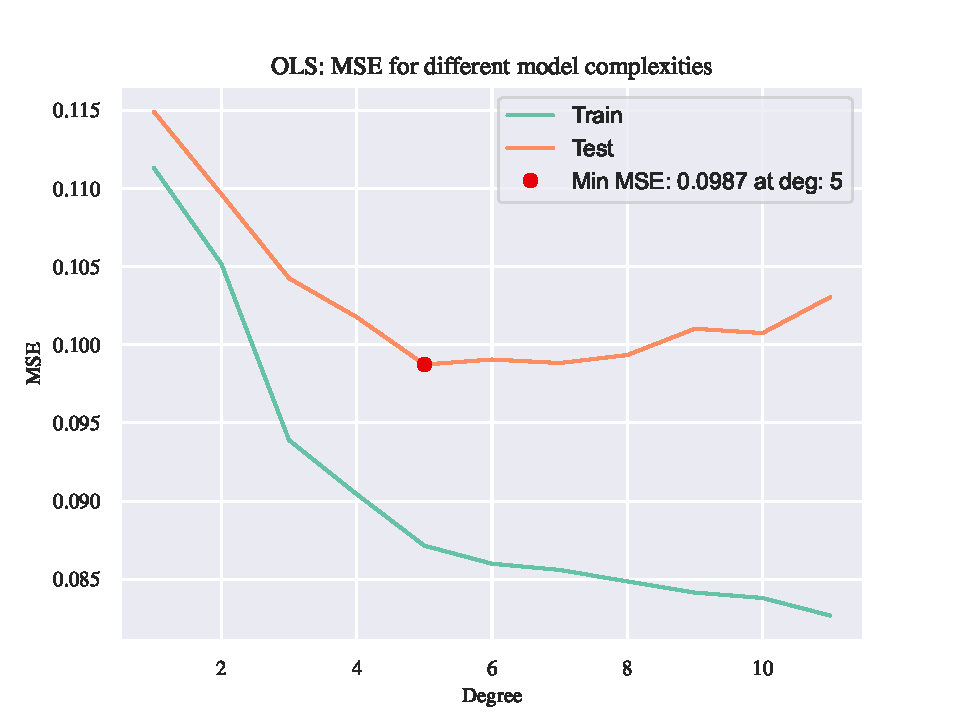
\includegraphics[width=1\linewidth]{project_1_alt/figures/figures_in_report/OLS_MSE_Franke_Noise.pdf}
    \caption{Mean squared error (MSE) for the ordinary least squares model both on training- and test data.}
    \label{fig:mseols}
\end{figure}

Fig. \ref{fig:mseols} shows how the mean square error (MSE) initially decreases as the degree of complexity increases. This seems reasonable as the Franke function makes up a complicated surface and one would think that higher degree polynomials are necessary to replicate it. 

We furthermore notice how the test error reaches its minimum at degree of complexity equal to 5. The test error increases as the polynomial degree further increases. We use the test error to choose the optimal degree of complexity. The training error continues to decrease. This is due to overfitting and the fact that OLS is designed to minimize the MSE. We use this as a sanity check of our model implementation.

\begin{figure}[h!]
    \centering
    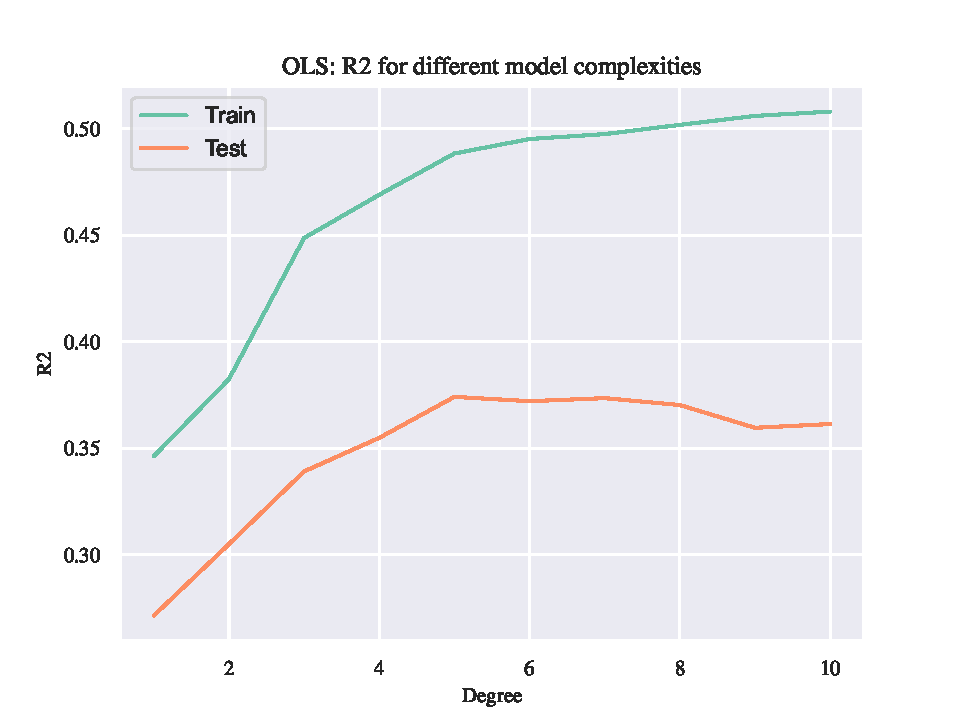
\includegraphics[width=1\linewidth]{project_1_alt/figures/figures_in_report/OLS_R2_Franke_Noise.pdf}
    \caption{$R^2$ for the ordinary least squares model both on training- and test data.}
    \label{fig:r2ols}
\end{figure}

The $R^2$ value increases as higher degree polynomials are introduced to the ordinary least squares model, as shown in Fig. \ref{fig:r2ols}. This is reasonable as we likely need higher degree polynomials to explain more variance in the data. The increase in $R^2$ halters at around degree equal to 10. At this point, introducing higher degree polynoimals does not help explain further variance in the data. The value of $R^2$ for the test data is lower then the one for the training data. This might be a sign that the model does not generalize well. 

\begin{figure}[h!]
    \centering
    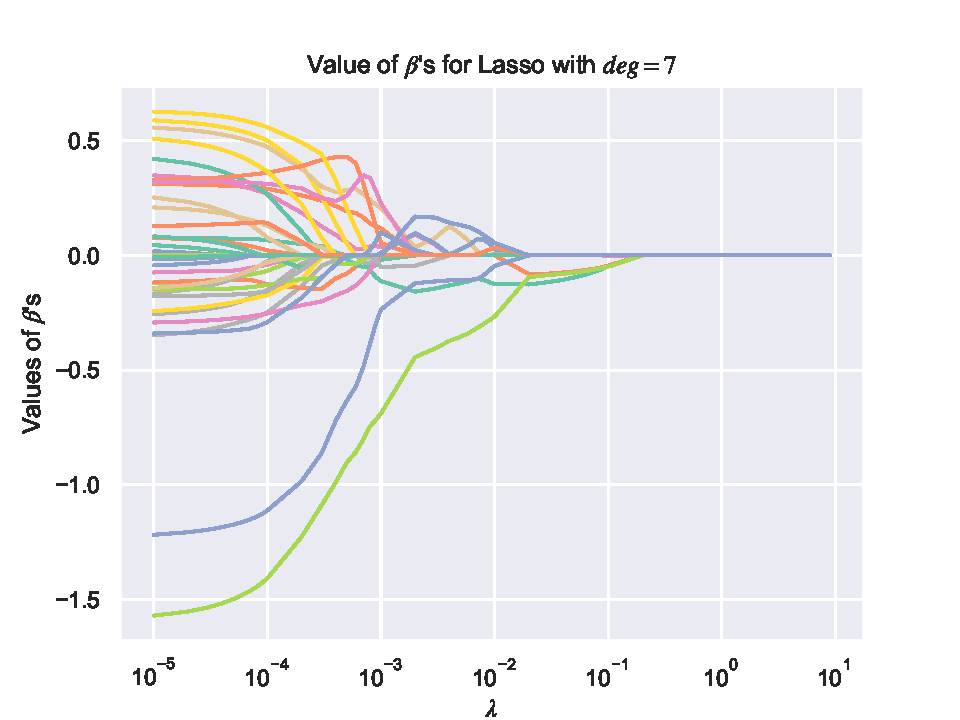
\includegraphics[width=1\linewidth]{project_1_alt/figures/figures_in_report/Ridge_Betas_lambda_Franke_Noise_const_deg.pdf}
    \caption{The values of the parameters $\bet$ for the ridge regression model with polynomials up to a degree of seven for increasing values of $\lambda$. Each colored line represents one $\beta_j$.}
    \label{fig:ridge_betas}
\end{figure}

\begin{figure}[h!]
    \centering
    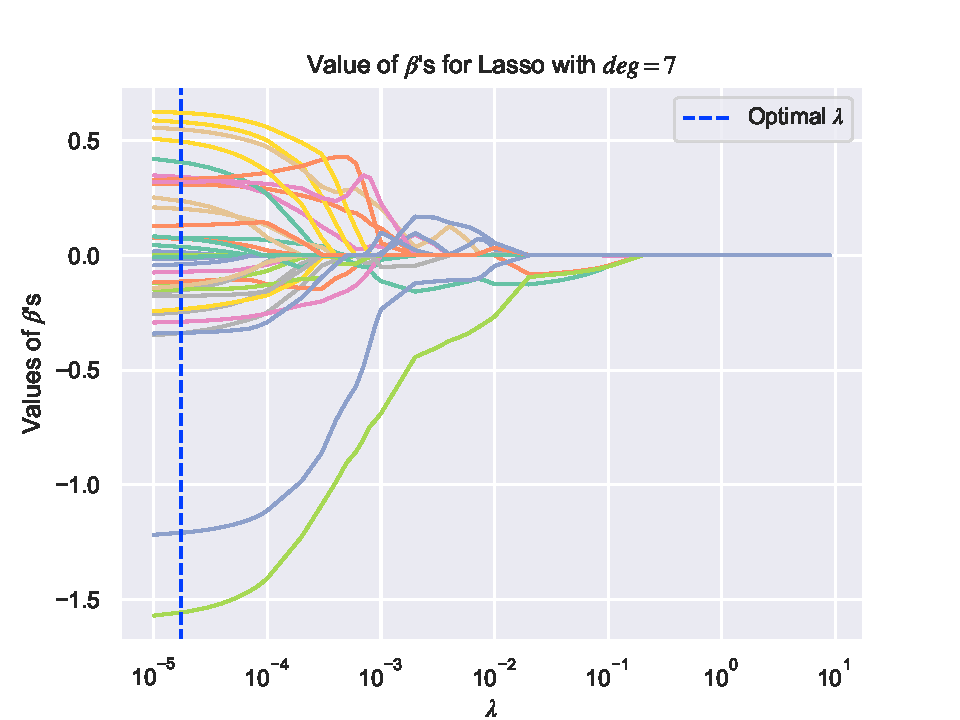
\includegraphics[width=1\linewidth]{project_1_alt/figures/figures_in_report/lasso_Betas_lambda_Franke_Noise_const_deg.pdf}
    \caption{The values of the parameters $\bet$ for the lasso regression model with polynomials up to a degree of seven for increasing values of $\lambda$. Each colored line represents one $\beta_j$.}
    \label{fig:lasso_betas}
\end{figure}

The $\bet$-values for our Ridge- and Lasso regression models are presented in Fig. \ref{fig:ridge_betas} and Fig. \ref{fig:lasso_betas} respectfully. For both models, we observe that the values of the coefficients are forced towards zero, and thereby also each other, as the penalty increases. For the Ridge regression coefficients, all have non-zero values regardless of the size of the penalty. For Lasso regression however, we observe that some are brought to zero at a sufficiently large penalty. Closer to $\lambda = 10^0 = 1$ all values of the $\beta$'s are brought to zero. A $\lambda$ value of this size seems highly unreasonable. 
The vertical line in each plot shows the optimal $\lambda$ in combination with the degree of complexity found through the grid search (numbers are available in Tab. \ref{tab:grid}). This backs up the claim that $\lambda$'s higher than 1 seem unreasonable. 

It is interesting to observe that the Lasso regression model has a far lower optimal $\lambda$-value than the Ridge regression model. It is important to note how the y-axis values in Fig. \ref{fig:ridge_betas} and in Fig. \ref{fig:lasso_betas} are different. The actual beta values chosen for the final model are comparable \mia{must check + elaborate}. 

\begin{figure}[h!]
    \centering
    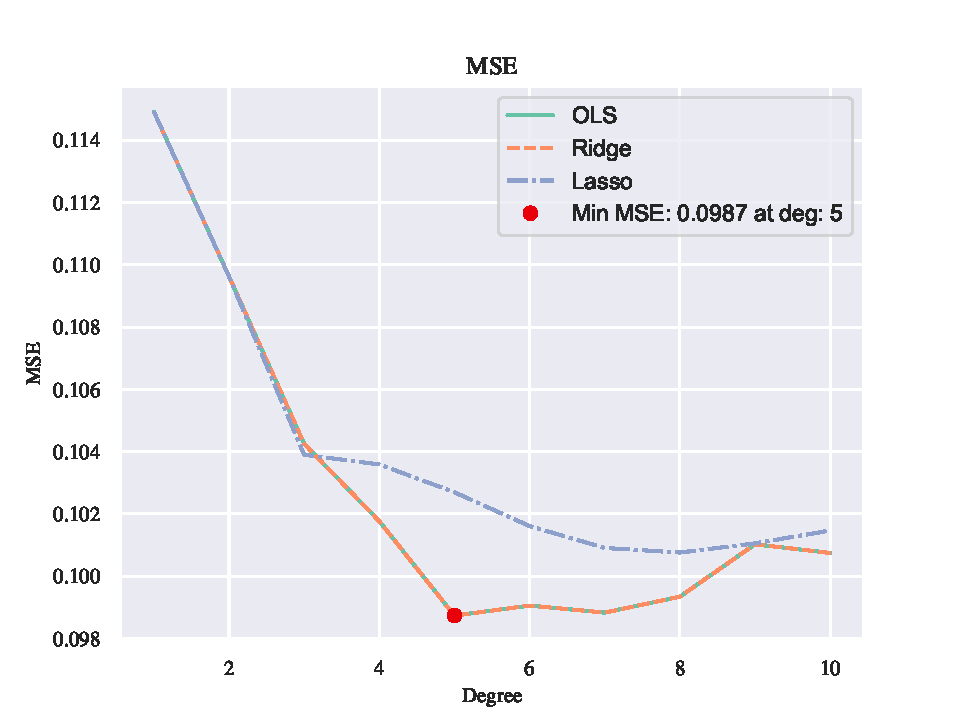
\includegraphics[width=1\linewidth]{project_1_alt/figures/figures_in_report/OLS_Ridge_Lasso_Franke_Noise.pdf}
    \caption{The MSE on the test data for OLS-, Ridge- and Lasso regression models. The minimum MSE is marked with a red dot.}
    \label{all3franke}
\end{figure}

We want to find the best model among OLS, Ridge and Lasso regression. In Fig. \ref{all3franke} we see the MSE on the test data for all three. OLS and Ridge far outperform Lasso regression. This may be due to \mia{?} The best model on the Franke function data is \mia{?}

\mia{why does Lasso suck?}

\begin{figure}
    \centering
    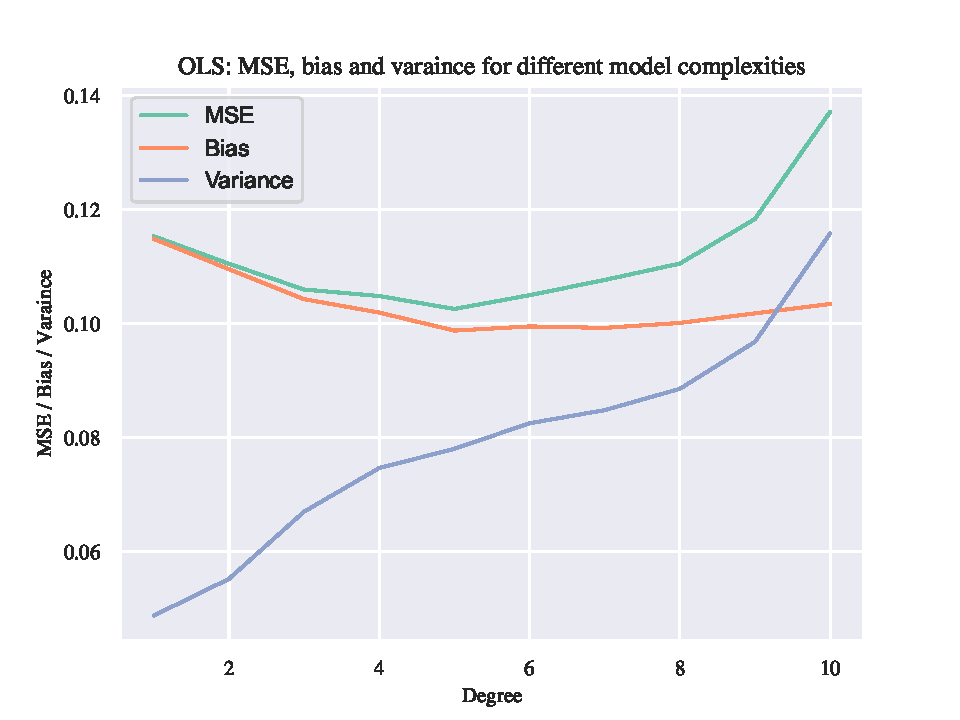
\includegraphics[width=1\linewidth]{project_1_alt/figures/figures_in_report/bias_var_Franke_Noise_bootstrap.pdf}
    \caption{MSE decomposed into a bias and a variance term for an ordinary least squares model trained with bootstrapping.
}
    \label{bias_var_trade}
\end{figure}

By using bootstrap samples, we have decomposed the MSE into a bias and a variance term for an OLS model. 
In Fig. \ref{bias_var_trade} the bias is initially high, but the variance is low. This is typical for an underfitted model. As the complexity increases, the bias goes down, whereas the variance increases. The lowest MSE is reached at some trade-off between the two. As the model complexity is further increased, the variance substantially increases and ensures an even higher MSE than at the beginning. This is a sign of an overfitted model.

\subsection{Terrain data}

\begin{figure}[h!]
    \centering
    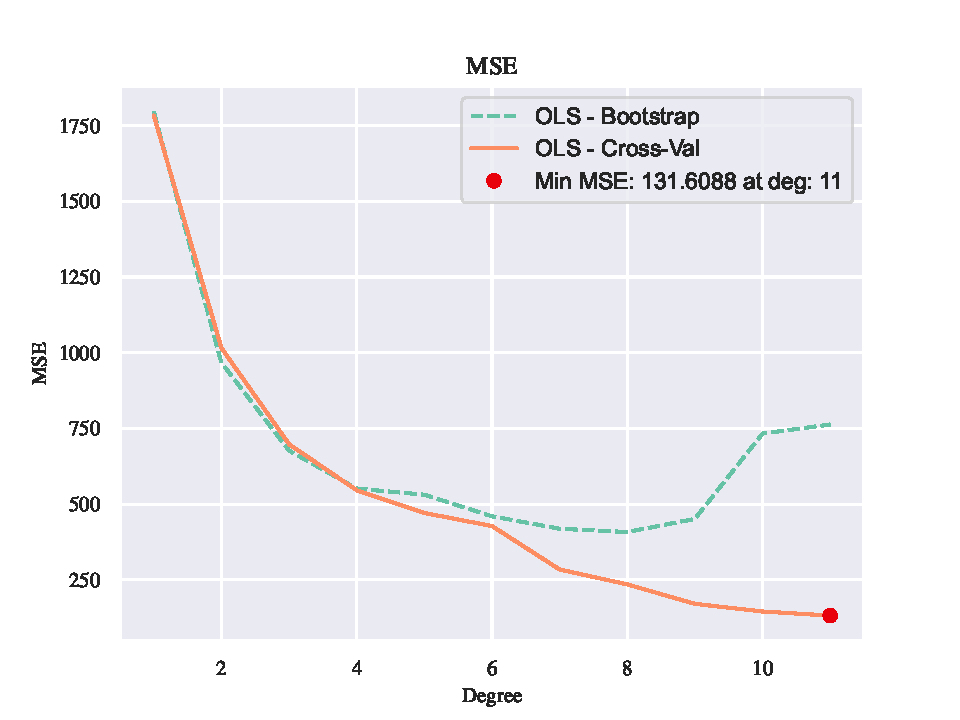
\includegraphics[width=1\linewidth]{project_1_alt/figures/figures_in_report/CV_BS_OLS_Terrain.pdf}
    \caption{MSE for three different models; OLS-, Ridge- and Lasso regression against degree of complexity. All are trained with cross-validation.}
    \label{cv_versus_bs}
\end{figure}

In Fig. \ref{cv_versus_bs} we compare bootstrapping to cross-validation. Both resampling techniques are used on the ordinary least squares model. The minimal MSE-value for the cross-validated OLS model is lower than for the bootstrapped model. The plot is not made for further degrees of complexity as we then reach problems with numerical precision (numbers lower than $\approx 10^{-15}$) and the MSE wrongly increases fast.  

There might be several reasons why the MSE is lower for cross-validation compared to bootstrapping. For the model trained with cross-validation, more data is utilized than for the one trained with bootstrap. In the ladder, we split into a training and a test data set, whereas cross-validation trains on the entire dataset.

We could have used the entire data set to draw bootstrap samples from. Then we would have to keep track of which samples were not included in the bootstrap sample and use these as the test set for the specific bootstrap model. This would allow us to use more data. This might be one of the reasons for the difference. \mia{what else?}


\begin{figure}[h!]
    \centering
    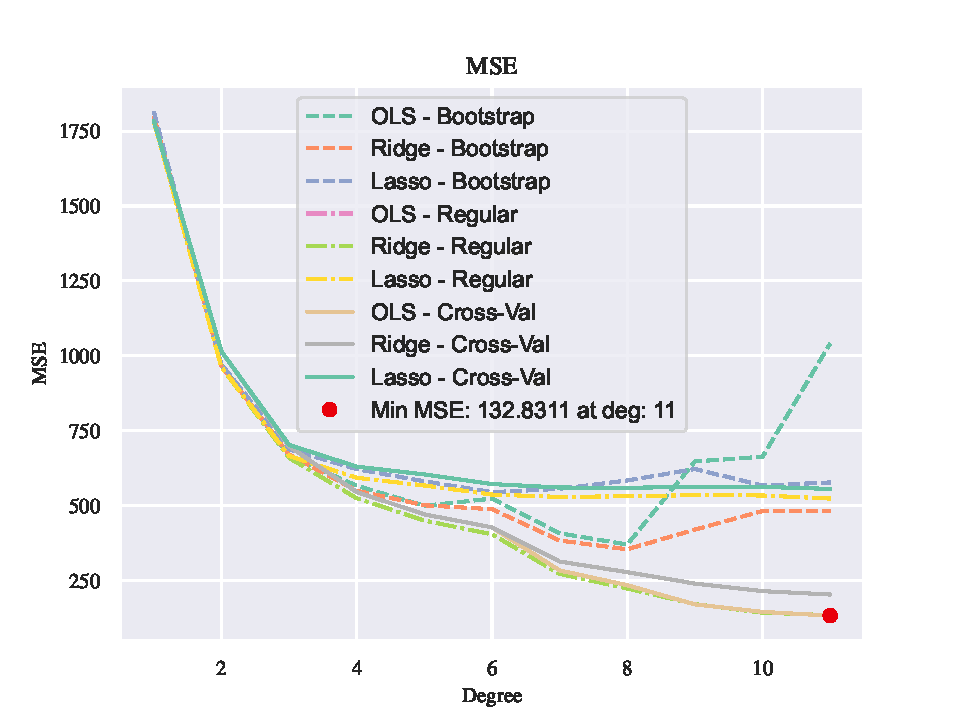
\includegraphics[width=1\linewidth]{project_1_alt/figures/figures_in_report/All_Terrain.pdf}
    \caption{MSE for OLS-, Ridge- and Lasso regression against degree of complexity. Each model is trained three times; with no resampling, using cross-validation and lastly, using bootstrapping. The minimum value for MSE is marked with a red dot.}
    \label{all_terrain}
\end{figure}

Our main goal is to find the very best model for terrain data. We have implemented three different model types; OLS, Ridge, and Lasso. Furthermore, we can use no resampling, bootstrapping or cross-validation. Combining this yields nine different models. In Fig. \ref{all_terrain} we compare the MSE on the test set for all. The two best models are Ridge regression with no resampling, as well as OLS with cross-validation. The ladder outperforms the former slightly and is therefore our best model. The lowest MSE is found at a degree of complexity of 11 and the MSE-value is approximately 134. As with Fig. \ref{cv_versus_bs}, this plot is only created for degrees of complexity up to 11 seeing as there are problems with numerical precision beyond this point. 

\mia{why is OLS CV best}

Choosing the number of data points for the terrain data was challenging. Including more data points meant having a dataset with more variance. This leads to models with a far higher MSE. 

Further work to do on this could include a different implementation of the bootstrap method.

Furthermore, it is interesting to discuss whether linear models are sufficient for these kinds of problems or not. \mia{continue + propose something else}

\mia{critical discussion of scaling of data must be included}